\id{IRSTI 06.35.01}{https://doi.org/10.58805/kazutb.v.4.25-541}

\begin{articleheader}
\sectionwithauthors{G.S.Tussibayeva, G.M.Sagindykova, A.E.Shakharova, U.B.Yussupov}{SPECTRAL ANALYSIS OF THE QUALITY OF THE AUDIT SERVICES MARKET}

{\bfseries \textsuperscript{1}G.S.Tussibayeva\textsuperscript{\envelope},
\textsuperscript{1}G.M.Sagindykova, \textsuperscript{2}A.E.Shakharova,
\textsuperscript{1}U.B.Yussupov}
\end{articleheader}

\begin{affiliation}

\textsuperscript{1}Kazakh University of Technology and Business, Astana,
Kazakhstan,

\textsuperscript{2}L.N.Gumilyov Eurasian National University, Astana,
Kazakhstan

\raggedright\textbf{\textsuperscript{\envelope}}Корреспондент-автор:\emph{igulmira\_80@mail.ru}
\end{affiliation}

The scientific article is aimed at studying a combination of qualitative
and quantitative methods to identify problems related to the audit
market, based on the analysis of interactions between all stakeholders
that can be applied to the market of audit and related services that
affect audit quality. General scientific and economic methods were
applied to comprehensively achieve the goals and objectives of the
research. The method of generalization allowed for a thorough analysis
of the material and the formation of the research structure, while the
interpretation and comparison methods helped assess the opinions of
researchers and identify the key features of the development of the
audit services market. A spectral analysis of the current audit services
market and system in Kazakhstan was conducted, allowing the evaluation
of the frequency characteristics of service quality over time or in
relation to other parameters. Based on data analysis and statistical
conclusions, findings about the current state of the audit services
market in the Republic of Kazakhstan were made, factors affecting
service quality were identified, and recommendations for improvement
were proposed. The results of the spectral analysis underwent
statistical processing, revealing significant patterns and differences
between various audit organizations and situations.

\textbf{Keywords:} audit, audit organization, audit services market,
audit service, professional audit organization, professional audit
activity council, audit quality.

\begin{articleheader}
{\bfseries АУДИТОРЛЫҚ ҚЫЗМЕТТЕР НАРЫҒЫНЫҢ САПАСЫН СПЕКТРЛІК ТАЛДАУ}

{\bfseries \textsuperscript{1} Г.С.Тусибаева\textsuperscript{\envelope},
\textsuperscript{1} Г.М.Сагиндыкова, \textsuperscript{2} А.Е. Шахарова,
\textsuperscript{1} У.Б. Юсупов}
\end{articleheader}

\begin{affiliation}

\textsuperscript{1}Қазақ технология және бизнес университеті, Астана қ.,
Қазақстан,

\textsuperscript{2}Л.Н. Гумилев атындағы Еуразия Ұлттық Университеті,
Астана қ., Қазақстан,

е-mail: igulmira\_80@mail.ru
\end{affiliation}

Ғылыми мақала аудит сапасына әсер ететін аудиторлық және ілеспе
қызметтер нарығына қолданылуы мүмкін, барлық мүдделі тараптар арасындағы
өзара іс-қимылды талдау негізінде аудиторлық нарықпен байланысты
проблемаларды айқындаудың сапалық және сандық әдістерінің кешенін
зерделеуге бағытталған\emph{.} Зерттеудің мақсаттары мен міндеттерін
жан-жақты жүзеге асыру үшін жалпы ғылыми және экономикалық әдістер
қолданылды. Жалпылау әдісі зерттеу материалына толық талдау жүргізуге
және зерттеудің құрылымын қалыптастыруға мүмкіндік берді. Ғалымдардың
пікірлерін бағалау және аудиторлық қызметтер нарығының даму
ерекшеліктерін анықтау үшін түсіндіру және салыстыру әдістері
пайдаланылды. Қазақстанның қазіргі аудиторлық қызметтер нарығы мен
жүйесіне спектрлік талдау жүргізілді, бұл қызметтердің сапасын уақыт пен
басқа параметрлерге байланысты бағалауға мүмкіндік берді. Мәліметтер мен
статистикалық қорытындыларды талдау негізінде Қазақстан Республикасының
аудиторлық қызметтер нарығының қазіргі жай-күйі туралы тұжырымдар
жасалды, қызмет сапасына әсер ететін факторлар анықталып, оны жақсарту
бойынша ұсыныстар берілді. Спектрлік талдау нәтижелері статистикалық
талдауға түсіп, әртүрлі аудиторлық ұйымдар мен жағдайлар арасындағы
маңызды заңдылықтар мен айырмашылықтар анықталды.

\textbf{Түйін сөздер:} аудит, аудиторлық ұйым, аудиторлық қызметтер
нарығы, аудиторлық қызмет, Кәсіби аудиторлық ұйым, аудиторлық қызмет
жөніндегі кәсіби кеңес, аудит сапасы.

\begin{articleheader}
{\bfseries СПЕКТРАЛЬНЫЙ АНАЛИЗ КАЧЕСТВА РЫНКА АУДИТОРСКИХ УСЛУГ}

{\bfseries \textsuperscript{1}Г.С.Тусибаева\textsuperscript{\envelope},
\textsuperscript{1}Г.М.Сагиндыкова, , \textsuperscript{2}А.Е.Шахарова,
\textsuperscript{1}У.Б.Юсупов}
\end{articleheader}

\begin{affiliation}

\textsuperscript{1}Казахский университет технологии и бизнеса, Астана,
Казахстан,

\textsuperscript{2}Евразийский национальный университет им.
Л.Н.Гумилева, Астана, Казахстан,

е-mail: igulmira\_80@mail.ru
\end{affiliation}

Научная статья направлена на изучение комплекса качественных и
количественных методов для определения проблем, связанных с аудиторским
рынком, на основе анализа взаимодействий между всеми заинтересованными
сторонами, которые могут быть применены к рынку аудиторских и
сопутствующих услуг, влияющих на качество аудита. Применение общенаучных
и экономических методов исследования способствует всесторонней
реализации поставленных целей и задач. Метод обобщения позволил детально
проанализировать материал и сформировать структуру исследования, а метод
интерпретации и сопоставления помог оценить мнения исследователей и
определить ключевые особенности развития аудиторского рынка. В ходе
исследования был проведен спектральный анализ казахстанского рынка
аудиторских услуг и его текущей системы, что позволило оценить частотные
характеристики качества услуг во временном разрезе и в зависимости от
других параметров. На основе анализа данных и статистических выводов
были сделаны заключения о состоянии рынка аудиторских услуг в Республике
Казахстан, выявлены факторы, влияющие на их качество, и даны
рекомендации по его улучшению. Результаты спектрального анализа были
подвергнуты статистической обработке, что позволило выявить значимые
закономерности и различия между аудиторскими организациями и ситуациями.

\textbf{Ключевые слова:} аудит, аудиторская организация, рынок
аудиторских услуг, аудиторская услуга, профессиональная аудиторская
организация, профессиональный совет по аудиторской деятельности,
качество аудита. 

\begin{multicols}{2}
\textbf{Introduction.} The audit market in Kazakhstan has recently faced
increasing instability, primarily due to a professional crisis within
the auditing sector. This has resulted in a significant decline in trust
towards audit institutions and practices. Various strategies to address
this crisis have emerged, focusing on the development of auditing
standards, heightened quality expectations for audit services, and the
creation of a robust system of professional values, ethics, and the
reputation of auditors. This includes self-regulating auditor
organizations and a comprehensive regulatory framework governing audit
activities.

By the late 1990s, the institutionalization of the audit profession was
completed, and its role within society became fully realized. All
subsequent developments have been shaped by two primary objectives:
ensuring high-quality professional services in line with business growth
and meeting the evolving needs of society.

Currently, the audit profession is evolving into a sector of socially
responsible business, where it offers assurance to stakeholders
regarding the reliability of business information, the accuracy of
financial statements, and the credibility of auditors and audit firms.

The importance of exploring the challenges and shifts within the audit
market is underscored by major transformations in the delivery of
professional audit services from 2013 to 2023. During this time, there
has been a notable change in the number of audit firms and Professional
Audit Organizations (PAOs) within Kazakhstan. These shifts are largely
driven by ongoing reforms within the audit industry and the broader
effects of economic crises and recovery periods. According to the
Quality Concept of Audit set by the International Auditing and Assurance
Standards Board (IAASB), changes in the audit market directly impact
service quality, necessitating a critical review of professional
practices. The goal is to identify additional methods for enhancing
audit quality within the professional landscape. This analysis uses a
spectral evaluation of the audit services market, particularly in light
of numerous scandals that have tarnished the profession and led to
growing dissatisfaction among consumers on a global scale.

\textbf{Literature Review}\emph{.} The review of literature on the audit
services market quality reveals the multifaceted nature of this subject,
involving elements such as professional standards, auditor independence
and impartiality, staff training and proficiency, internal quality
control systems, and the perspectives of stakeholders. Continuous
advancements in these areas are essential to maintaining the credibility
of financial reporting and the overall stability of financial markets.

Professional auditing standards, like the International Standards on
Auditing (ISA), are vital in ensuring high-quality audit services.
Studies indicate that adherence to these standards enhances the
transparency, reliability, and comparability of financial statements,
which is critical for fostering trust in corporate financial reports
(Tussibayeva G., Sagindykova G. 2023 {[}1{]}, Nurseitov E., Nurseitov D.
2016 {[}2{]}).

Stakeholder trust and perceptions of audit service quality, especially
from investors, creditors, regulators, and the general public, play a
crucial role. Research has shown that when trust in auditors and their
work is high, companies experience enhanced reputations, which boosts
their attractiveness to investors (Ernstberger J., Koch C., Schreiber E.
M., \& Trompeter G, 2020 {[}3{]}, Patrick Z, Vitalis K \& Mdoom I., 2017
{[}4{]}).

Various studies and articles examine the application of ISA across
different countries, including Kazakhstan. These works provide
analytical reviews, case studies, and discussions on errors and
improvements in the practical use of auditing standards (Kzykeeva A.S.,
Myrzakypova S.T., 2016 {[}5{]}, Xiao T, Geng C, \& Yuan C., 2020
{[}6{]}).

Additional research focuses on technological advancements, such as the
integration of data analytics and artificial intelligence in audit
procedures, which can significantly increase the efficiency and
precision of audits. Cultural and organizational factors impacting audit
service quality in Asia, along with potential strategies for
improvement, are also discussed (Noor A.S., Fatimah M.Y., Rusnah M.,
2018 {[}7{]}, Muhamad Taqi M., Rahmawati R., Bandi B., Murni S., \&
Warsina W., 2020 {[}8{]}).

Analyzing the experiences of regional integration organizations, such as
the European Union or Latin America, can offer valuable insights into
creating a unified audit services market within the EAEU. A unified
market would improve transparency and predictability in audit practices,
fostering greater investor confidence and reducing capital costs.
Studies explore the economic benefits and potential advantages of such a
market for business development in the region (Serov N. Yu., 2020
{[}9{]}, Kzykeyeva A., 2023 {[}10{]}).

\textbf{Materials and methods.} The research concentrated on exploring
both qualitative and quantitative methods for identifying issues within
the audit market, drawing on the historical development of the field as
discussed by scholars and incorporating recent studies by both
international and local researchers. Furthermore, a spectral analysis of
the audit services market was carried out, which examined the
interaction dynamics of various stakeholders involved in the audit and
related services markets, all of which influence audit quality.

The research methodology employed a range of approaches, including:

- Method of data collection and generalization: This approach enabled a
detailed analysis of the domestic audit services market, with a
particular focus on identifying key developmental challenges.

- Method of interpretation and comparison: Through inductive reasoning,
this method highlighted the strengths and weaknesses of self-regulation
within the auditing profession, influencing the application of the
quality concept at both audit firm and Professional Audit Organization
(PAO) levels.

- Method of analysis and synthesis: This method supported a
comprehensive evaluation of the audit services market\textquotesingle s
quality.

\textbf{Results and discussion.} In Kazakhstan, as in many parts of the
world, audit services are pivotal to modern economic development,
enhancing investment appeal by ensuring transparency and objectivity in
corporate reporting. The audit sector in Kazakhstan is a crucial part of
the financial system and the wider economy, playing a vital role in
maintaining the transparency, reliability, and stability of financial
structures, which in turn directly influences the investment
attractiveness of businesses in the Republic of Kazakhstan and the
country overall. In a rapidly evolving global economic environment and
with Kazakhstan striving for deeper integration into the global economy,
the advancement of the audit industry becomes increasingly significant.

The audit services market is expanding and evolving quickly. One of its
key features is the level of development and size of audit
organizations, with most large firms classified as growing entities.
Many of these firms have been established for years, while newer
companies are emerging with products and services offered both in
Kazakhstan and internationally {[}11{]}.

In Kazakhstan, the audit market includes the following types of
entities:

Four international firms known as the "Big Four":
PricewaterhouseCoopers, KPMG, Deloitte \& Touche, and Ernst \& Young;

Large domestic audit firms with substantial experience and smaller firms
with only a few employees;

Professional audit organizations and the Professional Council for
Auditing Activities.

Globally, the "Big Four" are recognized as the largest multinational
firms offering both audit and consulting services. This group includes
Ernst \& Young, Deloitte \& Touche, KPMG, and PricewaterhouseCoopers.
\end{multicols}

\begin{longtable}[]{|@{}
  >{\raggedright\arraybackslash}p{(\columnwidth - 6\tabcolsep) * \real{0.2521}}|@{}
  >{\raggedright\arraybackslash}p{(\columnwidth - 6\tabcolsep) * \real{0.2602}}|@{}
  >{\raggedright\arraybackslash}p{(\columnwidth - 6\tabcolsep) * \real{0.2457}}|@{}
  >{\raggedright\arraybackslash}p{(\columnwidth - 6\tabcolsep) * \real{0.2420}}|@{}}
  \caption*{Table 1- Quasi-Governmental Sector Companies Audited by Big-4}\\

  \hline
\begin{minipage}[b]{\linewidth}\raggedright
Ernst \& Young
\end{minipage} & \begin{minipage}[b]{\linewidth}\raggedright
PricewaterhouseCoopers
\end{minipage} & \begin{minipage}[b]{\linewidth}\raggedright
Deloitte
\end{minipage} & \begin{minipage}[b]{\linewidth}\raggedright
KPMG
\end{minipage} \\
\hline
\endhead
\hline
\endlastfoot
- Samruk-Kazyna Sovereign Wealth Fund;

- KazMunayGas (Exploration Production KMG, KazTransOil, KazTransGas, and
two refineries);

Kazakhtelecom;

Samruk-Kazyna Construction and United Chemical Company;

- Ekibastuz SDPS-2;

- KEGOC;

- KazAgro Holding;

- National Company "Kazakhstan Gharysh Sapary" & - Kazatomprom;

- Samruk-Energy;

- Samruk-Kazyna Invest;

- Zhilstroysberbank (now Otbas Bank);

- Kazakhstan Deposit Guarantee Fund & - UAPF (Unified Accumulative
Pension Fund);

- Kazakhstan Resilience Fund;

- Kazakhstan Temir Zholy group and its subsidiaries:

Kazakhstan Temir Zholy (national railway company)

KazTemirTrans (rail transport company)

Passenger Transportation

KTZ Freight Transportation

- Transtelecom;

- KTZ Express;

- Aktau Sea Trade Port;

- Kazatomprom & - Kazpost

- Air Astana

- Kazakhstan Airlines (Kazakhstani national carrier)

- Baiterek Holding

- Development Bank of Kazakhstan

- BRK-Leasing (now Industrial Development Fund)

- Kazakhstan Mortgage Company

- National Bank of Kazakhstan

- National Investment Corporation

- Astana Expo-2017

- KazAvtoZhol \\
\hline
\multicolumn{4}{|l|}{%
\emph{Note - compiled by the authors based on conducted research}} \\
\end{longtable}

\begin{multicols}{2}
As of 2024, these four firms employ a combined total of approximately
1.1 million people. Their collective revenues reach \$157 billion, with
the following breakdown (in billions of dollars): Deloitte - 47.60, PwC
- 43.03, EY- 37.20, KPMG- 29.22. Interestingly, these companies are
heavily involved in consulting as well. Of the total \$157 billion in
revenue, only \$57 billion is generated from audit services, with nearly
\$100 billion coming from consulting activities, particularly in tax
consulting.

These companies also operate nearly 3,000 offices worldwide. For
example, Ernst \& Young operates over 700 offices across more than 150
countries, while PwC has approximately 770 offices in 158 countries.
Most of these offices function as national legal entities or residents,
with some holding branch status under other resident companies.

While it is difficult to determine the exact market share of the Big
Four in Kazakhstan's audit sector, their influence is undeniable. These
firms audit nearly all major national companies, including banks,
pension funds, insurance companies, and oil firms. Table 1 lists the
quasi-public sector companies that are audited by the Big Four.

The audit services market in Kazakhstan has been experiencing dynamic
growth year after year. As a crucial component of the financial sector
and the national economy, it plays an essential role in maintaining the
transparency, reliability, and stability of the financial system, which
significantly influences the investment appeal of companies both within
Kazakhstan and throughout the country. Currently, the audit market in
Kazakhstan is represented by a considerable number of firms. Table 2
highlights the growth trends of audit firms between 2013 and 2023.
\end{multicols}

\begin{table}[H]
\caption*{Table 2 - The dynamics of the audit companies market, 2013-2023}
\centering
\resizebox{\textwidth}{!}{%
\begin{tabular}{|lccccccccccc|}
\hline
\multicolumn{1}{|c|}{\multirow{2}{*}{\begin{tabular}[c]{@{}c@{}}Regional \\ breakdown\end{tabular}}} &
  \multicolumn{11}{c|}{Number of audit firms} \\ \cline{2-12} 
\multicolumn{1}{|c|}{} &
  \multicolumn{1}{c|}{2013} &
  \multicolumn{1}{c|}{2014} &
  \multicolumn{1}{c|}{2015} &
  \multicolumn{1}{c|}{2016} &
  \multicolumn{1}{c|}{2017} &
  \multicolumn{1}{c|}{2018} &
  \multicolumn{1}{c|}{2019} &
  \multicolumn{1}{c|}{2020} &
  \multicolumn{1}{c|}{2021} &
  \multicolumn{1}{c|}{2022} &
  2023 \\ \hline
\multicolumn{1}{|l|}{Akmola Region} &
  \multicolumn{1}{c|}{1} &
  \multicolumn{1}{c|}{1} &
  \multicolumn{1}{c|}{1} &
  \multicolumn{1}{c|}{1} &
  \multicolumn{1}{c|}{2} &
  \multicolumn{1}{c|}{2} &
  \multicolumn{1}{c|}{4} &
  \multicolumn{1}{c|}{4} &
  \multicolumn{1}{c|}{3} &
  \multicolumn{1}{c|}{3} &
  5 \\ \hline
\multicolumn{1}{|l|}{Aktobe Region} &
  \multicolumn{1}{c|}{2} &
  \multicolumn{1}{c|}{2} &
  \multicolumn{1}{c|}{2} &
  \multicolumn{1}{c|}{3} &
  \multicolumn{1}{c|}{5} &
  \multicolumn{1}{c|}{6} &
  \multicolumn{1}{c|}{9} &
  \multicolumn{1}{c|}{9} &
  \multicolumn{1}{c|}{3} &
  \multicolumn{1}{c|}{5} &
  10 \\ \hline
\multicolumn{1}{|l|}{Almaty Region} &
  \multicolumn{1}{c|}{2} &
  \multicolumn{1}{c|}{2} &
  \multicolumn{1}{c|}{3} &
  \multicolumn{1}{c|}{3} &
  \multicolumn{1}{c|}{3} &
  \multicolumn{1}{c|}{4} &
  \multicolumn{1}{c|}{4} &
  \multicolumn{1}{c|}{4} &
  \multicolumn{1}{c|}{6} &
  \multicolumn{1}{c|}{5} &
  4 \\ \hline
\multicolumn{1}{|l|}{Atyrau Region} &
  \multicolumn{1}{c|}{-} &
  \multicolumn{1}{c|}{-} &
  \multicolumn{1}{c|}{-} &
  \multicolumn{1}{c|}{-} &
  \multicolumn{1}{c|}{-} &
  \multicolumn{1}{c|}{1} &
  \multicolumn{1}{c|}{3} &
  \multicolumn{1}{c|}{5} &
  \multicolumn{1}{c|}{15} &
  \multicolumn{1}{c|}{10} &
  10 \\ \hline
\multicolumn{1}{|l|}{East Kazakhstan Region} &
  \multicolumn{1}{c|}{2} &
  \multicolumn{1}{c|}{2} &
  \multicolumn{1}{c|}{2} &
  \multicolumn{1}{c|}{2} &
  \multicolumn{1}{c|}{2} &
  \multicolumn{1}{c|}{4} &
  \multicolumn{1}{c|}{4} &
  \multicolumn{1}{c|}{7} &
  \multicolumn{1}{c|}{2} &
  \multicolumn{1}{c|}{3} &
  7 \\ \hline
\multicolumn{1}{|l|}{Zhambyl Region} &
  \multicolumn{1}{c|}{2} &
  \multicolumn{1}{c|}{2} &
  \multicolumn{1}{c|}{2} &
  \multicolumn{1}{c|}{2} &
  \multicolumn{1}{c|}{2} &
  \multicolumn{1}{c|}{3} &
  \multicolumn{1}{c|}{3} &
  \multicolumn{1}{c|}{4} &
  \multicolumn{1}{c|}{2} &
  \multicolumn{1}{c|}{4} &
  4 \\ \hline
\multicolumn{1}{|l|}{West Kazakhstan Region} &
  \multicolumn{1}{c|}{1} &
  \multicolumn{1}{c|}{1} &
  \multicolumn{1}{c|}{1} &
  \multicolumn{1}{c|}{1} &
  \multicolumn{1}{c|}{1} &
  \multicolumn{1}{c|}{1} &
  \multicolumn{1}{c|}{1} &
  \multicolumn{1}{c|}{2} &
  \multicolumn{1}{c|}{1} &
  \multicolumn{1}{c|}{3} &
  3 \\ \hline
\multicolumn{1}{|l|}{Karaganda Region} &
  \multicolumn{1}{c|}{5} &
  \multicolumn{1}{c|}{5} &
  \multicolumn{1}{c|}{6} &
  \multicolumn{1}{c|}{7} &
  \multicolumn{1}{c|}{10} &
  \multicolumn{1}{c|}{13} &
  \multicolumn{1}{c|}{15} &
  \multicolumn{1}{c|}{18} &
  \multicolumn{1}{c|}{21} &
  \multicolumn{1}{c|}{20} &
  22 \\ \hline
\multicolumn{1}{|l|}{Kostanay Region} &
  \multicolumn{1}{c|}{2} &
  \multicolumn{1}{c|}{2} &
  \multicolumn{1}{c|}{2} &
  \multicolumn{1}{c|}{3} &
  \multicolumn{1}{c|}{3} &
  \multicolumn{1}{c|}{4} &
  \multicolumn{1}{c|}{5} &
  \multicolumn{1}{c|}{6} &
  \multicolumn{1}{c|}{8} &
  \multicolumn{1}{c|}{7} &
  8 \\ \hline
\multicolumn{1}{|l|}{Kyzylorda Region} &
  \multicolumn{1}{c|}{-} &
  \multicolumn{1}{c|}{-} &
  \multicolumn{1}{c|}{-} &
  \multicolumn{1}{c|}{-} &
  \multicolumn{1}{c|}{-} &
  \multicolumn{1}{c|}{1} &
  \multicolumn{1}{c|}{2} &
  \multicolumn{1}{c|}{5} &
  \multicolumn{1}{c|}{6} &
  \multicolumn{1}{c|}{5} &
  6 \\ \hline
\multicolumn{1}{|l|}{Mangystau Region} &
  \multicolumn{1}{c|}{1} &
  \multicolumn{1}{c|}{1} &
  \multicolumn{1}{c|}{1} &
  \multicolumn{1}{c|}{3} &
  \multicolumn{1}{c|}{3} &
  \multicolumn{1}{c|}{4} &
  \multicolumn{1}{c|}{5} &
  \multicolumn{1}{c|}{5} &
  \multicolumn{1}{c|}{1} &
  \multicolumn{1}{c|}{4} &
  4 \\ \hline
\multicolumn{1}{|l|}{Pavlodar Region} &
  \multicolumn{1}{c|}{1} &
  \multicolumn{1}{c|}{1} &
  \multicolumn{1}{c|}{1} &
  \multicolumn{1}{c|}{1} &
  \multicolumn{1}{c|}{1} &
  \multicolumn{1}{c|}{1} &
  \multicolumn{1}{c|}{2} &
  \multicolumn{1}{c|}{2} &
  \multicolumn{1}{c|}{2} &
  \multicolumn{1}{c|}{3} &
  4 \\ \hline
\multicolumn{1}{|l|}{North Kazakhstan Region} &
  \multicolumn{1}{c|}{2} &
  \multicolumn{1}{c|}{2} &
  \multicolumn{1}{c|}{2} &
  \multicolumn{1}{c|}{2} &
  \multicolumn{1}{c|}{2} &
  \multicolumn{1}{c|}{2} &
  \multicolumn{1}{c|}{4} &
  \multicolumn{1}{c|}{4} &
  \multicolumn{1}{c|}{1} &
  \multicolumn{1}{c|}{2} &
  2 \\ \hline
\multicolumn{1}{|l|}{Turkestan Region} &
  \multicolumn{1}{c|}{1} &
  \multicolumn{1}{c|}{1} &
  \multicolumn{1}{c|}{1} &
  \multicolumn{1}{c|}{1} &
  \multicolumn{1}{c|}{1} &
  \multicolumn{1}{c|}{1} &
  \multicolumn{1}{c|}{1} &
  \multicolumn{1}{c|}{1} &
  \multicolumn{1}{c|}{3} &
  \multicolumn{1}{c|}{3} &
  4 \\ \hline
\multicolumn{1}{|l|}{Abai Region} &
  \multicolumn{1}{c|}{} &
  \multicolumn{1}{c|}{} &
  \multicolumn{1}{c|}{} &
  \multicolumn{1}{c|}{} &
  \multicolumn{1}{c|}{} &
  \multicolumn{1}{c|}{} &
  \multicolumn{1}{c|}{} &
  \multicolumn{1}{c|}{} &
  \multicolumn{1}{c|}{} &
  \multicolumn{1}{c|}{3} &
  3 \\ \hline
\multicolumn{1}{|l|}{Zhetysu Region} &
  \multicolumn{1}{c|}{} &
  \multicolumn{1}{c|}{} &
  \multicolumn{1}{c|}{} &
  \multicolumn{1}{c|}{} &
  \multicolumn{1}{c|}{} &
  \multicolumn{1}{c|}{} &
  \multicolumn{1}{c|}{} &
  \multicolumn{1}{c|}{} &
  \multicolumn{1}{c|}{} &
  \multicolumn{1}{c|}{2} &
  3 \\ \hline
\multicolumn{1}{|l|}{Almaty City} &
  \multicolumn{1}{c|}{62} &
  \multicolumn{1}{c|}{67} &
  \multicolumn{1}{c|}{72} &
  \multicolumn{1}{c|}{79} &
  \multicolumn{1}{c|}{88} &
  \multicolumn{1}{c|}{112} &
  \multicolumn{1}{c|}{141} &
  \multicolumn{1}{c|}{161} &
  \multicolumn{1}{c|}{184} &
  \multicolumn{1}{c|}{197} &
  158 \\ \hline
\multicolumn{1}{|l|}{Astana City} &
  \multicolumn{1}{c|}{8} &
  \multicolumn{1}{c|}{10} &
  \multicolumn{1}{c|}{13} &
  \multicolumn{1}{c|}{19} &
  \multicolumn{1}{c|}{25} &
  \multicolumn{1}{c|}{39} &
  \multicolumn{1}{c|}{65} &
  \multicolumn{1}{c|}{92} &
  \multicolumn{1}{c|}{112} &
  \multicolumn{1}{c|}{125} &
  133 \\ \hline
\multicolumn{1}{|l|}{Shymkent City} &
  \multicolumn{1}{c|}{6} &
  \multicolumn{1}{c|}{6} &
  \multicolumn{1}{c|}{7} &
  \multicolumn{1}{c|}{8} &
  \multicolumn{1}{c|}{11} &
  \multicolumn{1}{c|}{15} &
  \multicolumn{1}{c|}{21} &
  \multicolumn{1}{c|}{24} &
  \multicolumn{1}{c|}{29} &
  \multicolumn{1}{c|}{30} &
  25 \\ \hline
\multicolumn{1}{|l|}{Total} &
  \multicolumn{1}{c|}{98} &
  \multicolumn{1}{c|}{\textit{105}} &
  \multicolumn{1}{c|}{116} &
  \multicolumn{1}{c|}{135} &
  \multicolumn{1}{c|}{159} &
  \multicolumn{1}{c|}{213} &
  \multicolumn{1}{c|}{289} &
  \multicolumn{1}{c|}{353} &
  \multicolumn{1}{c|}{410} &
  \multicolumn{1}{c|}{475} &
  417 \\ \hline
\multicolumn{12}{|l|}{\textit{Note - compiled by the authors based on conducted research}} \\ \hline
\end{tabular}}
\end{table}

\begin{multicols}{2}

The data presented in the tables highlight a substantial increase over
the past decade, suggesting a rising demand for audit services,
alongside enhancements in regulatory measures and market conditions for
these services. The majority of audit organizations are concentrated in
cities like Almaty, Astana, and Shymkent, which serve as major financial
and economic hubs. Across different regions of Kazakhstan, the growth of
audit organizations varies significantly.

The analysis indicates that the audit services market in Kazakhstan has
seen considerable expansion in several regions over the review period.
The highest growth rates were observed in key areas such as Almaty and
Astana, driven by investment activities and the development of vital
industries. Notable cities and industrial regions, including Karaganda
and Aktobe, are experiencing rapid growth, while some regions have shown
slower development. The expanding number of audit firms across the
country emphasizes the crucial role these services play in enhancing
transparency and economic efficiency.

As of 2023, there are 417 audit firms actively operating in Kazakhstan.
The majority of these firms are registered in Almaty, the financial hub,
with 208 firms (43.2\% of the total). Astana and Shymkent follow
closely, with 137 (28.5\%) and 27 (5.6\%) firms, respectively. While the
total number of audit firms stands at approximately 417, a more accurate
picture emerges when focusing on the "top twenty" firms, including the
Big Four---Deloitte \& Touche, Ernst \& Young, PricewaterhouseCoopers,
and KPMG---which adhere to specific quality standards and are authorized
to operate on the country\textquotesingle s stock exchange.

According to recent reports, only 24 audit firms, representing about 5\%
of the total, are included in the list of organizations recognized by
the Kazakhstan Stock Exchange (KASE). These firms are divided into two
levels based on their qualifications.

Level 1 consists of 13 firms, including "Russell Bedford A+ Partners"
LLP, "KPMG Audit" LLP, "PricewaterhouseCoopers" LLP, "Ernst \& Young"
LLP, "Deloitte" LLP, and several others like "Almir Consulting" LLP and
"Centraudit-Kazakhstan" LLP.

Level 2 includes 11 firms, such as "KoktemAudit" LLP, "MinTax Audit"
LLP, "Kazakhstanaudit" LLP, "Audit Company Solomon" LLP, and others like
"FinExpertiza Kazakhstan" LLP and "BDO Qazaqstan" LLP.

Despite this small group, the overall audit market in Kazakhstan has
shown dynamic growth year after year. According to the Chamber of
Auditors of the Republic of Kazakhstan, the audit market reached a
volume of 123.5 billion tenge in 2023, with the six largest
firms---KPMG, Deloitte, Ernst \& Young, PricewaterhouseCoopers, BDO
Kazakhstan, and Grant Thornton---accounting for 56\% of the market
share.

\end{multicols}

\begin{figure}[H]
	\centering
	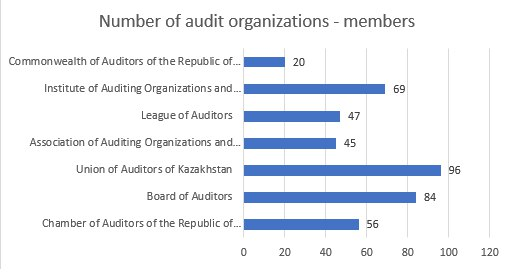
\includegraphics[width=0.6\textwidth]{media/ekon/image7.2}
	\caption*{Figure 1- Distribution of audit organizations by PJSC for 2023}
	\caption*{Note -- сompiled by the authors on the basis of past research}

\end{figure}

\begin{multicols}{2}

  A unique requirement for audit firms in Kazakhstan is membership in an
  accredited Professional Audit Organization (PAO), a non-profit entity
  that unites auditors and audit firms. Currently, there are seven
  registered PAOs in Kazakhstan, encompassing the 417 audit firms
  mentioned earlier (Figure 1).


The distribution of audit firms across Professional Audit Organizations
(PAO) in 2023 is as follows {[}11{]}:

Chamber of Auditors of the Republic of Kazakhstan: 56 firms

Collegium of Auditors: 84 firms

Union of Auditors of Kazakhstan: 96 firms

Association of Audit Organizations and Auditors of Kazakhstan: 45 firms

League of Auditors: 47 firms

Institute of Audit Organizations and Auditors of Kazakhstan: 69 firms

Commonwealth of Auditors of the Republic of Kazakhstan: 20 firms

According to the Ministry of Finance's digital platform, Kazakhstan
currently has over 1,600 auditors, with a notable rise in numbers over
the past few years. However, as reported by zakon.kz, a major issue in
the audit market has emerged due to the influx of auditors who lack
proper qualifications. Over the last two years alone, the number of
auditors increased by 1,300, a figure that surpasses the total growth
seen during the previous 25 years of the audit profession in Kazakhstan.

In terms of legal entities, only 18 out of the 417 audit firms in
Kazakhstan are part of the top 25 largest international audit networks.
Membership in these international networks allows firms to merge global
best practices with local expertise in providing audit services,
enhancing their reputation and establishing high standards of service.

Table 3 provides a breakdown of the membership of various audit
organizations across Kazakhstan\textquotesingle s regions, shedding
light on the regional distribution of auditors and the influence of
different professional associations on audit practices within the
country.

There are noticeable differences in the regional distribution of audit
organization memberships. For instance, the Chamber of Auditors of the
Republic of Kazakhstan and the Collegium of Auditors have a significant
presence in Almaty and Astana, while their membership numbers in other
regions are far lower, or these organizations may not be represented at
all.

The membership dynamics of different audit associations also vary across
regions over time. In Shymkent, for example, the League of Auditors and
the Association of Audit Organizations and Auditors of Kazakhstan have
seen a particularly strong increase in membership compared to other
regions.


Each of the listed audit organizations has distinct regional
distribution patterns, reflecting varied approaches to audit operations
and the recruitment of professionals.

In the first half of 2020, lawmakers and the Ministry of Finance in
Kazakhstan initiated amendments to legislation, which led to the
creation of the Professional Council for Audit Activities (PCAA), a
non-profit organization tasked with overseeing quality control and the
certification of auditors. The formation of the PCAA is intended to
align audit legislation with international standards, improving the
overall quality of audit services by implementing transparent
requirements for quality assurance and auditor certification {[}12{]}.

The Law of the Republic of Kazakhstan, "On Amendments and Additions to
Some Legislative Acts of the Republic of Kazakhstan on Audit Activities"
No. 358-VI, issued on July 3, 2020, establishes the PCAA as a
non-membership, non-profit organization created by professional bodies.
The council\textquotesingle s goal is to "enhance the
state\textquotesingle s economic policy" and to provide independent
oversight aimed at protecting investors. Representatives from
Kazakhstan's Ministry of Finance will be part of the council's board.
Additionally, representatives from KASE, the MFCA administration,
auditors, and others will also be involved.
\end{multicols}

\begin{table}[H]
  \caption*{Table 3 - Distribution of audit firms by professional audit
organizations in the regional context, 2023}
\centering
\resizebox{\textwidth}{!}{%
\begin{tabular}{|lccccccc|}
\hline
\multicolumn{1}{|c|}{Regional section} &
  \multicolumn{1}{c|}{\begin{tabular}[c]{@{}c@{}}Chamber of \\ Auditors of \\ the Republic\\  of Kazakhstan\end{tabular}} &
  \multicolumn{1}{c|}{\begin{tabular}[c]{@{}c@{}}Board of\\  Auditors\end{tabular}} &
  \multicolumn{1}{c|}{\begin{tabular}[c]{@{}c@{}}Union of\\  Auditors of\\ Kazakhstan\end{tabular}} &
  \multicolumn{1}{c|}{\begin{tabular}[c]{@{}c@{}}Institute of\\  Auditing\\ Organizations \\ and Auditors \\ of Kazakhstan\end{tabular}} &
  \multicolumn{1}{c|}{\begin{tabular}[c]{@{}c@{}}League of \\ Auditors\end{tabular}} &
  \multicolumn{1}{c|}{\begin{tabular}[c]{@{}c@{}}Association \\ of Auditing \\ Organizations \\ and Auditors \\ of Kazakhstan\end{tabular}} &
  \begin{tabular}[c]{@{}c@{}}Commonwealth \\ of Auditors of\\  the Republic \\ of Kazakhstan\end{tabular} \\ \hline
\multicolumn{1}{|l|}{Kazakhstan} &
  \multicolumn{1}{c|}{56} &
  \multicolumn{1}{c|}{84} &
  \multicolumn{1}{c|}{96} &
  \multicolumn{1}{c|}{45} &
  \multicolumn{1}{c|}{47} &
  \multicolumn{1}{c|}{69} &
  20 \\ \hline
\multicolumn{1}{|l|}{Akmola region} &
  \multicolumn{1}{c|}{2} &
  \multicolumn{1}{c|}{1} &
  \multicolumn{1}{c|}{-} &
  \multicolumn{1}{c|}{-} &
  \multicolumn{1}{c|}{-} &
  \multicolumn{1}{c|}{1} &
  1 \\ \hline
\multicolumn{1}{|l|}{Aktobe region} &
  \multicolumn{1}{c|}{1} &
  \multicolumn{1}{c|}{1} &
  \multicolumn{1}{c|}{-} &
  \multicolumn{1}{c|}{2} &
  \multicolumn{1}{c|}{5} &
  \multicolumn{1}{c|}{-} &
  1 \\ \hline
\multicolumn{1}{|l|}{Almaty region} &
  \multicolumn{1}{c|}{1} &
  \multicolumn{1}{c|}{-} &
  \multicolumn{1}{c|}{1} &
  \multicolumn{1}{c|}{-} &
  \multicolumn{1}{c|}{1} &
  \multicolumn{1}{c|}{-} &
  1 \\ \hline
\multicolumn{1}{|l|}{Almaty} &
  \multicolumn{1}{c|}{31} &
  \multicolumn{1}{c|}{43} &
  \multicolumn{1}{c|}{44} &
  \multicolumn{1}{c|}{14} &
  \multicolumn{1}{c|}{18} &
  \multicolumn{1}{c|}{5} &
  3 \\ \hline
\multicolumn{1}{|l|}{Astana} &
  \multicolumn{1}{c|}{12} &
  \multicolumn{1}{c|}{26} &
  \multicolumn{1}{c|}{20} &
  \multicolumn{1}{c|}{22} &
  \multicolumn{1}{c|}{10} &
  \multicolumn{1}{c|}{36} &
  7 \\ \hline
\multicolumn{1}{|l|}{Atyrau region} &
  \multicolumn{1}{c|}{-} &
  \multicolumn{1}{c|}{1} &
  \multicolumn{1}{c|}{2} &
  \multicolumn{1}{c|}{1} &
  \multicolumn{1}{c|}{2} &
  \multicolumn{1}{c|}{3} &
  1 \\ \hline
\multicolumn{1}{|l|}{\begin{tabular}[c]{@{}l@{}}East Kazakhstan\\  region\end{tabular}} &
  \multicolumn{1}{c|}{2} &
  \multicolumn{1}{c|}{1} &
  \multicolumn{1}{c|}{1} &
  \multicolumn{1}{c|}{1} &
  \multicolumn{1}{c|}{-} &
  \multicolumn{1}{c|}{-} &
  2 \\ \hline
\multicolumn{1}{|l|}{Zhambyl region} &
  \multicolumn{1}{c|}{1} &
  \multicolumn{1}{c|}{-} &
  \multicolumn{1}{c|}{-} &
  \multicolumn{1}{c|}{-} &
  \multicolumn{1}{c|}{1} &
  \multicolumn{1}{c|}{2} &
  - \\ \hline
\multicolumn{1}{|l|}{\begin{tabular}[c]{@{}l@{}}West Kazakhstan \\ region\end{tabular}} &
  \multicolumn{1}{c|}{1} &
  \multicolumn{1}{c|}{-} &
  \multicolumn{1}{c|}{2} &
  \multicolumn{1}{c|}{-} &
  \multicolumn{1}{c|}{-} &
  \multicolumn{1}{c|}{-} &
  - \\ \hline
\multicolumn{1}{|l|}{Karaganda region} &
  \multicolumn{1}{c|}{1} &
  \multicolumn{1}{c|}{1} &
  \multicolumn{1}{c|}{14} &
  \multicolumn{1}{c|}{-} &
  \multicolumn{1}{c|}{1} &
  \multicolumn{1}{c|}{5} &
  - \\ \hline
\multicolumn{1}{|l|}{Kostanay region} &
  \multicolumn{1}{c|}{-} &
  \multicolumn{1}{c|}{5} &
  \multicolumn{1}{c|}{-} &
  \multicolumn{1}{c|}{2} &
  \multicolumn{1}{c|}{-} &
  \multicolumn{1}{c|}{-} &
  1 \\ \hline
\multicolumn{1}{|l|}{Kyzylorda region} &
  \multicolumn{1}{c|}{1} &
  \multicolumn{1}{c|}{1} &
  \multicolumn{1}{c|}{2} &
  \multicolumn{1}{c|}{-} &
  \multicolumn{1}{c|}{1} &
  \multicolumn{1}{c|}{1} &
  - \\ \hline
\multicolumn{1}{|l|}{Mangystau region} &
  \multicolumn{1}{c|}{1} &
  \multicolumn{1}{c|}{1} &
  \multicolumn{1}{c|}{-} &
  \multicolumn{1}{c|}{-} &
  \multicolumn{1}{c|}{-} &
  \multicolumn{1}{c|}{1} &
  1 \\ \hline
\multicolumn{1}{|l|}{Abai region} &
  \multicolumn{1}{c|}{-} &
  \multicolumn{1}{c|}{2} &
  \multicolumn{1}{c|}{1} &
  \multicolumn{1}{c|}{-} &
  \multicolumn{1}{c|}{-} &
  \multicolumn{1}{c|}{-} &
  - \\ \hline
\multicolumn{1}{|l|}{Jetysui region} &
  \multicolumn{1}{c|}{-} &
  \multicolumn{1}{c|}{-} &
  \multicolumn{1}{c|}{-} &
  \multicolumn{1}{c|}{-} &
  \multicolumn{1}{c|}{2} &
  \multicolumn{1}{c|}{-} &
  1 \\ \hline
\multicolumn{1}{|l|}{Atyrau region} &
  \multicolumn{1}{c|}{-} &
  \multicolumn{1}{c|}{-} &
  \multicolumn{1}{c|}{-} &
  \multicolumn{1}{c|}{-} &
  \multicolumn{1}{c|}{-} &
  \multicolumn{1}{c|}{-} &
  - \\ \hline
\multicolumn{1}{|l|}{Pavlodar region} &
  \multicolumn{1}{c|}{-} &
  \multicolumn{1}{c|}{-} &
  \multicolumn{1}{c|}{2} &
  \multicolumn{1}{c|}{1} &
  \multicolumn{1}{c|}{-} &
  \multicolumn{1}{c|}{1} &
  - \\ \hline
\multicolumn{1}{|l|}{\begin{tabular}[c]{@{}l@{}}North Kazakhstan\\  region\end{tabular}} &
  \multicolumn{1}{c|}{-} &
  \multicolumn{1}{c|}{-} &
  \multicolumn{1}{c|}{-} &
  \multicolumn{1}{c|}{-} &
  \multicolumn{1}{c|}{-} &
  \multicolumn{1}{c|}{2} &
  - \\ \hline
\multicolumn{1}{|l|}{Turkestan region} &
  \multicolumn{1}{c|}{-} &
  \multicolumn{1}{c|}{-} &
  \multicolumn{1}{c|}{1} &
  \multicolumn{1}{c|}{1} &
  \multicolumn{1}{c|}{-} &
  \multicolumn{1}{c|}{2} &
  - \\ \hline
\multicolumn{1}{|l|}{Shymkent} &
  \multicolumn{1}{c|}{2} &
  \multicolumn{1}{c|}{1} &
  \multicolumn{1}{c|}{6} &
  \multicolumn{1}{c|}{1} &
  \multicolumn{1}{c|}{6} &
  \multicolumn{1}{c|}{8} &
  1 \\ \hline
\multicolumn{8}{|l|}{\textit{Note - compiled by the authors on the basis of the conducted research}} \\ \hline
\end{tabular}%
}
\end{table}

\begin{multicols}{2}


The new council will set the standards for audit firms conducting
mandatory audits of KASE-listed organizations, MFCA, national management
holdings, national companies, and subsoil users. Furthermore, the
council will be responsible for auditing firms\textquotesingle{} quality
checks, addressing complaints about auditors, approving external quality
control procedures, and coordinating auditor candidate certifications.

Many within the auditing community are skeptical about the new body's
effectiveness, particularly because the quality control of audit
services by the council is not governed by the Entrepreneurial Code of
the Republic of Kazakhstan. This creates a situation where audit firms
may not be able to defend their rights under the law, potentially
increasing corruption risks.

According to the PAO "Collegium of Auditors," the creation of this new
body may result in a loss of client trust in auditors. Given that
Kazakhstan is part of the Eurasian Economic Council (EAEU) and an
agreement has been signed for a unified audit market within the EAEU,
clients may seek audit services in Russia or Kyrgyzstan if the situation
in Kazakhstan's audit market worsens.

A similar reform in Russia led to a reduction of 600 audit firms between
2018 and 2020, while the number of auditors with the right to perform
mandatory audits dropped by 76\%. Gulmira Zhamukhanbetova, Executive
Director of the PAO "Institute of Audit Organizations and Auditors of
Kazakhstan," has noted that amendments to the Law "On Audit Activities"
have created operational challenges for audit firms. For instance,
amendments did not clarify whether qualifications issued to auditors
before July 6 remain valid. Consequently, auditors are now required to
undergo certification by the qualification commission of the council,
but such certified auditors currently do not exist in Kazakhstan, and no
certifications have been conducted since July 6, 2021.

Thus, the establishment of the Professional Council for Audit Activities
is a contentious issue. On one hand, the council is aimed at raising
audit service quality, globally recognizing Kazakhstani audit reports,
introducing corporate governance methods, and improving Kazakhstan's
investment appeal through transparent financial reporting. On the other
hand, there is concern that audits could fall under governmental
control, from the approval of audit licenses to the audit processes
themselves, which may lead to market monopolization by a select group of
companies.

It is also important to mention that soon, Kazakhstani auditors will be
able to work freely across EAEU countries, as Kazakhstan ranks second
after Russia in the number of audit organizations. On April 19, 2022,
the EAEU Agreement on Audit Activities was signed in Moscow {[}13{]},
and it came into effect on May 26, 2023, following ratification by all
member countries: Belarus (September 20, 2022), Armenia (November 16,
2022), Kyrgyzstan (January 11, 2023), Kazakhstan (October 4, 2023), and
Russia (April 26, 2023). The agreement facilitates the creation of a
single audit market within the EAEU, allowing audit firms from any
member country to operate throughout the Union. Audit reports produced
in one EAEU country will be accepted across the Union {[}13{]}. Unified
standards for audit practices, audit firms, and auditors will be
implemented.

Within the context of the EAEU, Kazakhstan\textquotesingle s audit
services market is competitive, represented by 417 firms and 1,500
auditors. In comparison, Russia had 2,700 authorized audit firms at the
end of 2022, down from 4,200 in 2020, with 16,400 auditors. In Belarus,
the number of audit firms decreased from 67 to 63 in 2022, while the
number of individual auditors dropped from 286 to 262, and certified
auditors from 1,321 to 1,224, reflecting a 7.3\% decrease.

Establishing a unified market is a complex, long-term process requiring
the collaboration of all EAEU member states. Key issues being addressed
include differences in national audit legislation, the lack of a unified
audit regulation system, underdeveloped infrastructure, and the shortage
of qualified personnel {[}14{]}. In conclusion, the audit markets in
Kazakhstan and the EAEU are undergoing active development and
modernization, creating new opportunities for audit firms and
contributing to a more favorable investment environment. Additionally,
the EAEU audit services market, especially in Kazakhstan, is projected
to grow at a faster rate than the global market, though the region still
lags behind in the adoption and integration of AI into the audit
workspace compared to global trends.

In summary, the research has identified several problematic areas in the
self-regulation of the audit services market in Kazakhstan:

Inability to objectively assess financial reporting quality: There is a
risk that management or staff within audit organizations may engage in
actions or inaction that compromise the objectivity of financial
reporting assessments.

Non-compliance with regulations: Many audit organizations fail to comply
fully or appropriately with the legal framework that governs the audit
market.

Weaknesses in the regulatory framework: There is a lack of robust
methodologies and approaches to external quality control, which
currently relies heavily on formalities and selective document reviews
by auditors rather than a comprehensive audit quality analysis.

Public Audit Organizations (PAOs) struggling with responsibilities: PAOs
are unable to adequately fulfill their roles in coordinating the audit
market and overseeing external quality control, and there is an absence
of a risk-oriented approach to external audits to address industry
dumping.

Lack of a long-term strategy for audit organizations: Particularly for
small and medium-sized firms, there is no clear development strategy for
the medium or long term.

Concealment of illegal actions: Some audit organizations may hide
unlawful practices by the audited entities in order to retain contracts
and clients.

Reluctance to provide financial statements for voluntary audits: There
is often hesitation on the part of entities to submit financial
statements for voluntary audits.

Abolition of auditor confidentiality: This undermines trust and
transparency in audit processes.

Introduction of criminal liability for auditors: This presents
significant legal risks for auditors and may deter professionals from
performing their duties effectively.

These issues prevent the proper implementation of the quality concept in
auditing, both at the level of individual audit firms and PAOs.

To address these challenges, the following measures are recommended to
reduce the risks of compromising the quality of professional activities:

Revise quality assessment practices: The current methods, focused on
standard compliance, are becoming outdated and are contributing to a
crisis within the audit industry. A review and update of these practices
are needed.

Eliminate excessive regulatory requirements: Reducing unnecessary
demands on the audit business will help improve the professional quality
of services.

Implement anti-dumping strategies: PAOs and industry regulators should
introduce measures to combat dumping in the professional audit market.

Adjust PAO methods for evaluating audit efficiency: PAOs need to revise
how they assess auditor efficiency and ensure that fees align with the
scope and duration of audit services. This may involve an overhaul of
the entire pricing system for audit firms.

Develop new PAO control mechanisms: PAOs should introduce additional
tools to enforce accountability, especially regarding violations of the
Code of Professional Ethics for Auditors and the Rules of Independence.
In the long term, these measures should help balance audit pricing with
the costs incurred by audit organizations, including personnel,
programs, and control mechanisms.

Improving the quality of auditing in a professional environment as a
multifaceted process includes improving the methodology of audit work,
professional development of specialists, the introduction of modern
technologies and control methods.

A key factor in improving quality is the continuous training of auditors
and their professional development. This includes both regular updating
of accounting knowledge and new legislative initiatives, as well as
obtaining professional certifications such as CPA or ACCA. The
independence of the auditor is also one of the fundamental principles on
which a quality audit is based. In order to maintain objectivity and
impartiality in the audit process, it is necessary to ensure the
auditor\textquotesingle s independence from both the client and personal
interests.

Risk management is also an important element. Auditors should carefully
assess the risks at each stage of the audit and determine which areas of
reporting require the most attention. To do this, it is necessary to use
modern risk management systems that help identify potentially
problematic areas and focus efforts on their analysis. The introduction
of such tools can significantly improve the efficiency of audit work.
Modern technologies, including big data analysis, artificial
intelligence and automation of routine processes, also play an important
role in improving audit quality. Data analysis software, such as tools
such as IDEA and ACL, allows auditors to more quickly detect anomalies
and errors that might have been overlooked with the traditional
verification method. Automating repetitive tasks reduces the burden on
auditors and helps them focus on more complex and important aspects of
the audit.

An important aspect is also the organization of interaction with the
client. Regular communication with the management of the organization
helps the auditor to better understand the specifics of the business and
take into account the possible risks associated with its activities.
Clear and timely interaction helps to prevent misunderstandings and
timely identify potential problems in reporting. To improve the quality
of work, it is also important to monitor the implementation of standards
within the audit organization itself. The implementation of an internal
quality control system, as well as regular internal audits of the
auditors\textquotesingle{} work, help identify inconsistencies and
errors at an early stage, which contributes to improving the final
result. In addition, external quality control conducted by regulatory
authorities plays an important role in maintaining a high level of
professionalism and in preventing possible violations.

Thus, improving the quality of audit requires an integrated approach,
including improving methodology, training specialists, using modern
technologies and ensuring strict control at all stages of work. This
helps to increase the reliability of financial reports and strengthen
trust in the auditing profession as a whole.

\textbf{Conclusions.} The audit services sector in Kazakhstan is a
regulated market overseen by state authorities, legal frameworks, and
accredited organizations. This segment is continuously evolving to meet
global standards while addressing the specific needs of the national
economy. The involvement of international network representatives
enhances the appeal and competitiveness of the market. The growth of
Kazakhstan\textquotesingle s audit services market has led to the
strengthening of both market and government regulation. Increased
competition among audit firms, the introduction of new audit services,
the establishment of audit associations focused on service quality
control, and the development of new auditing standards---closely aligned
with international norms---are all key drivers of this progress.
Additionally, the legislative framework has also evolved alongside these
developments. Looking forward, the ongoing expansion of the audit
services market will further amplify the role of state regulation.
Continuous legislative updates and increased government oversight will
be essential to ensuring high-quality audit services.

Improving the quality of the audit is critical to ensure the reliability
of financial statements, increase the confidence of investors and other
stakeholders, as well as to minimize risks and prevent financial losses.
A high-quality audit contributes to compliance with the law, improving
the company\textquotesingle s reputation, and improving the
effectiveness of internal control and corporate governance. It also
plays a key role in reducing the cost of capital and supporting
strategic decision-making. Ultimately, improving the quality of audit
contributes to the sustainability of the business, its competitiveness
and the growth of trust in financial markets.
\end{multicols}

\begin{center}
  {\bfseries References}
\end{center}
  
\begin{references}

1. Tussibayeva G.S., Sagindykova G.M. Osnovy i procedury audita v
sootvetstvii s mezhdunarodnymi \\standartami audita. Uchebnik (UMO RUMS
MON RK). - Almaty: TOO «Izdatel\textquotesingle stvo LEM», 2023. - 340
b. ISBN 978-601-239-743-7 {[}in Russian{]}

2.Nurseitov Je. Nurseitov D. Glavnaja kniga auditora. Posobie po
mezhdunarodnym standartam audita, dejstvujushhim v RK: TOO
«Izdatel\textquotesingle stvo «LEM», 2016.- 426 s. ISBN 9786018023910

{[}in Russian{]}

3. Ernstberger J., Koch C., Schreiber E. M., \& Trompeter G Are audit
firms\textquotesingle{} compensation policies associated with audit
quality? //Contemporary Accounting Research. -2020. - Vol.37(1). -P.
218-244. \href{https://DOI/}{DOI} 10.1111/1911-3846.12528

4.Patrick Z, Vitalis K \& Mdoom I. Effect of auditor independence on
audit quality: A review of literature// International Journal of
Business and Management Invention. -2017. -Vol. 6 (3). -P. 51-59.

5.Kzykeeva A.S., Myrzhakypova S.T. Analiz kachestva audita v uslovijah
kazahstanskogo rynka// The Journal of Economic Research \& Business
Administration.- Vol.2(128). -2019. - S.131-138. DOI
\\10.26577/be.2019.v128.i2.012 {[}in Russian{]}

6.Xiao T, Geng C, \& Yuan C. "How audit effort affects audit quality: An
audit process and audit output perspective"// China Journal of
Accounting Research. -2020.-Vol. 13(1). -P. 109-127.

DOI 10.1016/j.cjar.2020.02.002

7.Noor A.S., Fatimah M.Y., Rusnah M. Perspectives on audit quality: An
analysis // Asian Journal of Accounting Perspectives. -2018. -Vol.
11(1).-P. 1-27. DOI10.22452/AJAP.vol11no1.1 {[}in Russian{]}

8.Muhamad Taqi M., Rahmawati R., Bandi B., Murni S., \& Warsina W. Audit
Quality Attributes and Client Factors // AFRE (Accounting and Financial
Review). -2020.-Vol.3(1).- P.1-13. DOI 10.26905/afr.v3i1.3884

9. Serov N. Ju. Voprosy konkurencii v ramkah sozdanija edinogo rynka
auditorskih uslug v EAJeS / N. Ju. Serov. - Tekst: neposredstvennyj //
Molodoj uchenyj. - 2020. - № 30 (320). - S. 121-124.
\\https://moluch.ru/archive/320/72804 {[}in Russian{]}

10.Kzykeyeva A. Risk-Based Approach to Improving the Quality of Internal
Audit// Quality - Access to Success. -2022. - Vol.23(189). -P. 228-237.
DOI 10.47750/QAS/23.189.26

11.Auditorskij rynok Kazahstana na pod\#jome: obzor situacii. ---
{[}Jelektronnyj resurs{]}.URL:
\\\href{https://ranking.kz/reviews/banking-and-finance/auditorskiy-rynok-kazahstana-na-podyome-obzor-situatsii.html}{https://ranking.kz}
(Data obrashhenija: 20.06.2024). {[}in Russian{]}

12.Professional\textquotesingle nyj sovet po auditorskoj
dejatel\textquotesingle nosti. - {[}Jelektronnyj resurs{]}. URL:
https://psad.kz (Data obrashhenija: 24.06.2024). {[}in Russian{]}

13.O ratifikacii Soglashenija ob osushhestvlenii auditorskoj
dejatel\textquotesingle nosti v ramkah Evrazijskogo \\jekonomicheskogo
sojuza. - {[}Jelektronnyj resurs{]}. URL:
https://adilet.zan.kz/rus/docs/Z2300000041\textbackslash{} (Data
obrashhenija: 27.06.2024). {[}in Russian{]}

14.Formirovanie edinyh rynkov uslug EAJeS v oblasti audita, sostavlenija
otchetnosti i buhgalterskogo ucheta.
URL:https://eec.eaeunion.org/comission/department (Data obrashhenija:
26.06.2024). {[}in Russian{]}
\end{references}

\begin{authorinfo}
\hspace{1em}\emph{\textbf{Information about the authors}}

Tussibayeva G.S. - Ph.D, Associate Professor, Kazakh University of
Technology and Business, Astana, Kazakhstan, e-mail:
igulmira\_80@mail.ru;

Sagyndykova G. M. - Candidate of Economics, Associate Professor, Kazakh
University of Technology and Business, Astana, Kazakhstan, e-mail:
gsmaktobe1@mail.ru;

Shakharova A.Ye. - Candidate of Economics, Associate Professor, L.N.
Gumilyov Eurasian National University, Astana, Kazakhstan, e-mail:
shaharovaaliya@yandex.kz;

Yusupov U.B. \textbf{-} Ph.D, Associate Professor, Kazakh University of
Technology and Business, Astana, Kazakhstan, e-mail: \\nusup86@mail.ru

\hspace{1em}\emph{\textbf{Сведения об авторах}}

Тусибаева Г.С.\textbf{-} Ph.D, ассоциированный профессор, Казахский
университет технологии и бизнеса, г. Астана, Казахстан. e-mail:
igulmira\_80@mail.ru;

Сагиндыкова Г. М.- к.э.н., ассоциированный профессор, Казахский
университет технологии и бизнеса, г. Астана, Казахстан. e-mail:
gsmaktobe1@mail.ru;

Шахарова А.Е.- .э.н., доцент, Евразийский национальный университет имени
Л.Н. Гумилева, г. Астана, Казахстан. e-mail: shaharovaaliya@yandex.kz;

Юсупов У.Б.- Ph.D, ассоциированный профессор, Казахский университет
технологии и бизнеса, г. Астана, Казахстан. e-mail: nusup86@mail.ru;
\end{authorinfo}
